\chapter{Beta machine, CPU design}

As explained in the introduction, the goal of this work is to design a Beta machine. This machine is 
in fact a minimalist CPU based on the Harvard architecture, i.e. data and intructions are stored in 
two different memories. The machine uses words of 32 bits, represented in small endians, 
and only implements operations of 2's complement signed integers. 

In this section the different modules making up the Beta machine are studied one by one, from 
their functionality to their design. Simulation results are even provided for some of them. Once the 
different elements are explained, the desired instruction set for the Beta machine is
described. And finally, the different modules are connected to each other to form the Beta
machine with the desired instruction set.

\section{Beta machine components}

\subsection{Program counter}

The program counter is a module with seven inputs (clk, clk\_en, rst, pcsel, offset, data, pc\_in) 
and two outputs (pc\_out and pc\_next), as shown in Figure \ref{fig:components/pc}. 
Its functions are to provide the current counter on pc\_out ($PC$) and its 
next value ($PC + 4$) on pc\_next, and to react to a control signal named pcsel. This control 
allows to choose the program counter's operating mode. The different modes and their functions
are listed in Table \ref{tab:pc/modes}. Note that if one connects pc\_new to pc\_in and that pcsel
is set to 0b00, the program counter acts like a simple 32bits 4-by-4 counter.

\begin{figure}[H]
    \centering
    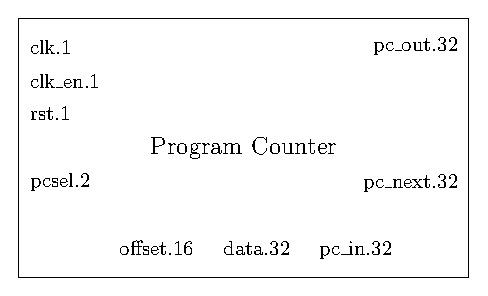
\includegraphics[scale=0.8]{Chapter3-CPU/res/pc}
    \caption{Program Counter}
    \label{fig:components/pc}
\end{figure}

\begin{table}[ht]
    \centering
    \begin{tabular}{|l|l|l|}
    \hline
    \rowcolor[HTML]{DAE8FC} 
    \multicolumn{1}{|c|}{\cellcolor[HTML]{DAE8FC}\textbf{Mode}} & \multicolumn{1}{c|}{\cellcolor[HTML]{DAE8FC}\textbf{pcsel}} & \multicolumn{1}{c|}{\cellcolor[HTML]{DAE8FC}\textbf{Details}}                                                                                                                                                                       \\ \hline
    NORMAL                                                      & 0b00                                                        & \begin{tabular}[c]{@{}l@{}}The current value of the counter program pc\_out becomes \\ the value taken from the input pc\_in.\end{tabular}                                                                                          \\ \hline
    BEQ                                                         & 0b01                                                        & \begin{tabular}[c]{@{}l@{}}The current value of the counter program pc\_out becomes \\ the value taken on the input pc\_in if the value on data is not 0. \\ Otherwise, the current value becomes pc\_in + 4 $\times$ offset.\end{tabular} \\ \hline
    JMP                                                         & 0b10                                                        & \begin{tabular}[c]{@{}l@{}}The current value of the counter program pc\_out becomes the \\ value on data.\end{tabular}                                                                                                              \\ \hline
    BNE                                                         & 0b11                                                        & \begin{tabular}[c]{@{}l@{}}The current value of the counter program pc\_out becomes\\  the value taken on the input pc\_in if the value on data is 0. \\ Otherwise, the current value becomes pc\_in + 4 $\times$ offset.\end{tabular}     \\ \hline
    \end{tabular}
    \caption{Program counter modes}
    \label{tab:pc/modes}
\end{table}

Concerning the internal circuit (that is shown in Figure \ref{fig:components/pc_in}), the pc\_out 
values is evaluated for the different modes and 
is put on a multiplexer which chooses the right output according to the pcsel value. For the BNE 
and BEQ modes, another multiplexer is used to make the selection between the two possible results, 
the control of these two multiplexers is naturally done by the result of $data == 0$. 

For the offset, it should be noted that it first undergoes a conversion from signed 16bits to 
signed 32bits before actually being used in the circuit.

The result selected by the multiplexer controlled by pcsel then goes to the register where it is 
stored at the next rising edge of the clock if the clk\_enable is high. The 
pc\_out thus has the desired value and the pc\_next simply corresponds to pc\_out + 4. When 
the reset (rst) is high, the register is synchronously reset to 0.

\begin{figure}[H]
    \centering
    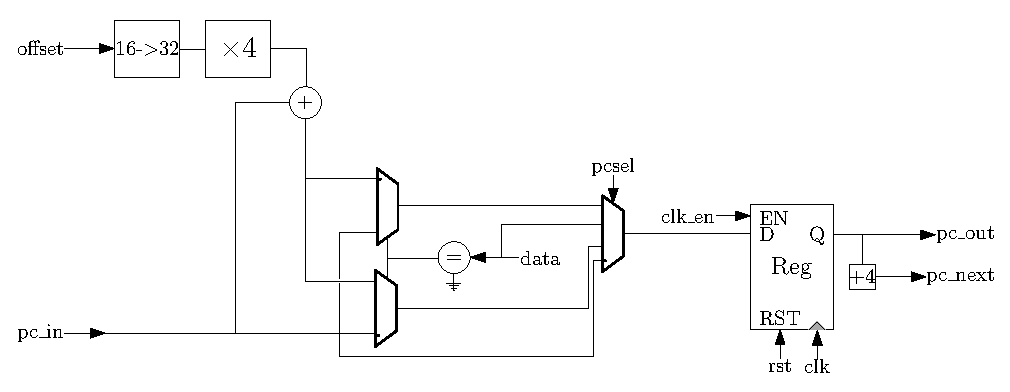
\includegraphics[width=\linewidth]{Chapter3-CPU/res/pc_internal}
    \caption{Program Counter internal circuit}
    \label{fig:components/pc_in}
\end{figure}

The Verilog implementation of the program counter is not a problem. Everything is relatively 
straight-forward for this module.

\subsubsection*{Program counter simulations}

The different modes of the program counter have been verified by simulation. In the first mode 
(NORMAL mode, pcsel = 0b00), it was checked that with a pc\_in at 4 294 967 292 (the maximum value with 
the last two bits at 0 that helds on 32 bits), the program counter returned 0 for pc\_next and did not 
give a random value. Other random values for pc\_in were checked to be sure that it worked 
correctly. Results of this first simulation are shown in Figure \ref{fig:sim/pc_00}. Note that the
input values are changed only once per two clock cycles but the module is totally able to manage
input changes once per cycle.

\begin{figure}[H]
    \centering
    \includegraphics[width=\linewidth]{Chapter3-CPU/res/pc_simu_00.PNG}
    \caption{Program Counter in normal mode simulations for various pc\_in values}
    \label{fig:sim/pc_00}
\end{figure}

To test the JMP mode (pcsel = 0b10), it was simply tried to set data to several values to check if 
pc\_out became this value. Results are provided in Figure \ref{fig:sim/pc_10}.

\begin{figure}[H]
    \centering
    \includegraphics[width=\linewidth]{Chapter3-CPU/res/pc_simu_10.PNG}
    \caption{Program Counter in jmp mode simulations for various data values}
    \label{fig:sim/pc_10}
\end{figure}

The last simulation was for the BEQ (pcsel = 01) and BNE (pcsel = 11) modes in order to check 
different offsets (positive and negative) with data fixed at a certain value and then at 0.
Results are given in Figure \ref{fig:sim/pc_01} for BEQ and \ref{fig:sim/pc_11} for BNE.

\begin{figure}[H]
    \centering
    \includegraphics[width=\linewidth]{Chapter3-CPU/res/pc_simu_01.PNG}
    \caption{Program Counter in BEQ mode simulations for various data and offset values}
    \label{fig:sim/pc_01}
\end{figure}

\begin{figure}[H]
    \centering
    \includegraphics[width=\linewidth]{Chapter3-CPU/res/pc_simu_11.PNG}
    \caption{Program Counter in BNE mode simulations for various data and offset values}
    \label{fig:sim/pc_11}
\end{figure}

In the different simulations the results are all valid, which adds confidence to this design before 
moving on to the practical implementation that comes later.

\subsection{ALU}

The Arithmetic Logic Unit (ALU) allows the resolution of arithmetic, logic and bit shifting 
operations. These operations are selected using the alufn signal. The chosen operation is then 
applied on the two operands data\_a and data\_b and sends the result on res. The different 
operations are listed in Table \ref{tab:alu/alufn}\footnote{unsigned(data\_b[4:0]) in the table means 
that only the five last bits of data\_b are used and that they are intepreted as an unsigned number
}and a view of the module is shown in Figure \ref{fig:components/alu}. 

\begin{figure}[ht]
    \centering
    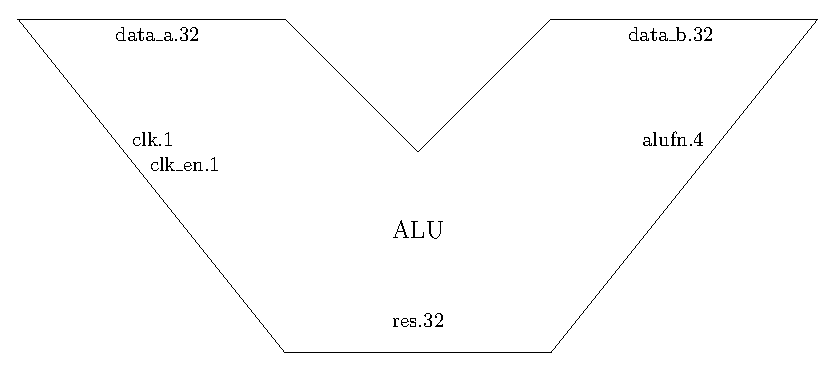
\includegraphics[scale=0.8]{Chapter3-CPU/res/alu}
    \caption{Arithmetic Logic Unit (ALU)}
    \label{fig:components/alu}
\end{figure}

\begin{table}[ht]
    \centering
    \begin{tabular}{|l|l|l|}
    \hline
    \rowcolor[HTML]{DAE8FC} 
    \multicolumn{1}{|c|}{\cellcolor[HTML]{DAE8FC}\textbf{Operation}} & \multicolumn{1}{c|}{\cellcolor[HTML]{DAE8FC}\textbf{alufn}} & \multicolumn{1}{c|}{\cellcolor[HTML]{DAE8FC}\textbf{Result}}   \\ \hline
    No operation                                                     & 0b0000                                                      & res = 0                                                        \\ \hline
    Addition                                                         & 0b0001                                                      & res = data\_a + data\_b                                        \\ \hline
    Substraction                                                     & 0b0010                                                      & res = data\_a - data\_b                                        \\ \hline
    Multiplication                                                   & 0b0011                                                      & res = data\_a $\times$ data\_b                    \\ \hline
    No operation                                                     & 0b0100                                                      & res = 0                                                        \\ \hline
    Bitwise-and                                                      & 0b0101                                                      & res = data\_a \& data\_b                                       \\ \hline
    Bitwise-or                                                       & 0b0110                                                      & res = data\_a $|$ data\_b                                        \\ \hline
    Bitwise-xor                                                      & 0b0111                                                      & res = data\_a $\oplus$ data\_b                         \\ \hline
    Compare equal                                                    & 0b1000                                                      & res = (data\_a == data\_b) ? 1 : 0                             \\ \hline
    Compare less                                                     & 0b1001                                                      & res = (data\_a \textless data\_b) ? 1 : 0                      \\ \hline
    Compare less or equal                                            & 0b1010                                                      & res = (data\_a $\leq$ data\_b) ? 1 : 0                   \\ \hline
    Logical left shift                                               & 0b1011                                                      & res = data\_a $<<$ unsigned(data\_b[4:0])                     \\ \hline
    Logical right shift                                              & 0b1100                                                      & res = data\_a $>>$ unsigned(data\_b[4:0])               \\ \hline
    Arithmetic right shift                                           & 0b1101                                                      & res = data\_a $>>>$ unsigned(data\_b[4:0]) \\ \hline
    No operation                                                     & 0b1110                                                      & res = 0                                                        \\ \hline
    No operation                                                     & 0b1111                                                      & res = 0                                                        \\ \hline
    \end{tabular}
    \caption{ALU operations}
    \label{tab:alu/alufn}
\end{table}

Regarding the internal design of the ALU shown in Figure \ref{fig:components/alu_in}, it is very 
simple. Indeed, all the operations are executed in parallel and a multiplexer is in charge of 
selecting the result that is transmitted to the output. This value is then recorded in the 
register on the rising edge of the clock if the clk\_en is in the high state. For the ALU, there is 
no reset, that's why the register reset is always 0.

\begin{figure}[H]
    \centering
    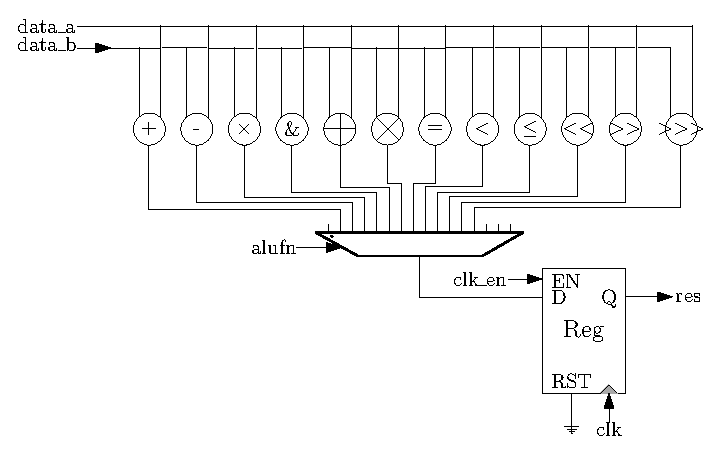
\includegraphics[width=\linewidth]{Chapter3-CPU/res/alu_internal}
    \caption{Arithmetic Logic Unit (ALU) internal circuit}
    \label{fig:components/alu_in}
\end{figure}


For the implementation of the ALU in Verilog, the operators are directly used in the code and the 
compiler selects the right circuits to perform them. The arithmetic operations are 
performed by DSPs while the logic operations are performed directly by logic gates. Concerning the
shifts, they are basically free on an FPGA. Indeed, shifting the 
connections of the signals is enough to achieve it, that does not pose any concern.

\subsubsection*{ALU simulations}

In order to check the behavior of the ALU, all the operations have been tested with different 
operands : the tested combinations data\_a, data\_b are listed in Table \ref{tab:alu/sim}. 
All the results obtained are correct, which validates the ALU.

\begin{table}[H]
    \centering
    \begin{tabular}{|l|l|}
    \hline
    \rowcolor[HTML]{DAE8FC} 
    \multicolumn{1}{|c|}{\cellcolor[HTML]{DAE8FC}\textbf{data\_a}} & \multicolumn{1}{c|}{\cellcolor[HTML]{DAE8FC}\textbf{data\_b}} \\ \hline
    800                                                            & 8                                                             \\ \hline
    0                                                              & 0                                                             \\ \hline
    0                                                              & 8                                                             \\ \hline
    8                                                              & 0                                                             \\ \hline
    -1                                                             & 8                                                             \\ \hline
    8                                                              & -1                                                            \\ \hline
    -8                                                             & 8                                                             \\ \hline
    8                                                              & -8                                                            \\ \hline
    \end{tabular}
    \caption{Operand combinations used in the ALU simulations}
    \label{tab:alu/sim}
\end{table}

The results of the simulations are shown in Figures \ref{fig:sim/alu_0} to \ref{fig:sim/alu_7}.

\begin{figure}[H]
    \centering
    \includegraphics[width=\linewidth]{Chapter3-CPU/res/alu_simu_0.PNG}
    \caption{ALU simulations for alufn = 0b0000 (No operation), 0b0001 (Addition), 0b0010 (Substraction) 
    and 0b0011 (Multiplication). data\_a, data\_b and res values are shown in signed decimal 
    representation}
    \label{fig:sim/alu_0}
\end{figure}

\begin{figure}[H]
    \centering
    \includegraphics[width=\linewidth]{Chapter3-CPU/res/alu_simu_1_0.PNG}
    \caption{ALU simulations for alufn = 0b0100 (No op) and 0b0101 (Bitwise-and). data\_a, data\_b and
    res values are shown in hexadecimal representation}
    \label{fig:sim/alu_1}
\end{figure}

\begin{figure}[H]
    \centering
    \includegraphics[width=\linewidth]{Chapter3-CPU/res/alu_simu_1_1.PNG}
    \caption{ALU simulations for alufn = 0b0110 (Bitwise-or) and 0b0111 (Bitwise-xor). data\_a, data\_b and
    res values are shown in hexadecimal representation}
    \label{fig:sim/alu_2}
\end{figure}

\begin{figure}[H]
    \centering
    \includegraphics[width=\linewidth]{Chapter3-CPU/res/alu_simu_2.PNG}
    \caption{ALU simulations for alufn = 0b1000 (Compare equal), 0b1001 (Compare less) and
    0b1010 (Compare less equal). data\_a, data\_b and res values are shown in signed decimal 
    representation}
    \label{fig:sim/alu_3}
\end{figure}

\begin{figure}[H]
    \centering
    \includegraphics[width=\linewidth]{Chapter3-CPU/res/alu_simu_3_0.PNG}
    \caption{ALU simulations for alufn = 0b1011 (Logical left shift). data\_a and
    res values are shown in hexadecimal representation. data\_b is shown in signed decimal 
    representation}
    \label{fig:sim/alu_4}
\end{figure}

\begin{figure}[H]
    \centering
    \includegraphics[width=\linewidth]{Chapter3-CPU/res/alu_simu_3_1.PNG}
    \caption{ALU simulations for alufn = 0b1100 (Logical right shift). data\_a and
    res values are shown in hexadecimal representation. data\_b is shown in signed decimal 
    representation}
    \label{fig:sim/alu_5}
\end{figure}

\begin{figure}[H]
    \centering
    \includegraphics[width=\linewidth]{Chapter3-CPU/res/alu_simu_3_2.PNG}
    \caption{ALU simulations for alufn = 0b1101 (Arithmetic right shift). data\_a and
    res values are shown in hexadecimal representation. data\_b is shown in signed decimal 
    representation}
    \label{fig:sim/alu_6}
\end{figure}

\begin{figure}[H]
    \centering
    \includegraphics[width=\linewidth]{Chapter3-CPU/res/alu_simu_4.PNG}
    \caption{ALU simulations for alufn = 0b1110 (No operation) and 0b1111 (No operation).
     data\_a, data\_b and res values are shown in signed decimal 
    representation}
    \label{fig:sim/alu_7}
\end{figure}

\subsection{Memories, generalities}

On the Cyclone V, all memory definitions are done through the same interface: the altsyncrams. 
Whether it is for RAM, ROM, one port, two ports, two real ports (independent clocks), ... this 
module is used. Also, both MLAB and M10K are represented by this Verilog module. 
Obviously, for all these different functions, the module must be configured. This is done on 
the one hand by a parameterization (for example to specify the size of the memory, the size of the 
words, the choice of the type MLAB or M10K, the number of ports, of clocks, the inputs / outputs 
which are registered, if there is a clock enable or not, ...) and on the other hand by the inputs 
and outputs which are used or not (for example for the ROM all the ports linked to the writing is not 
used and the write enable is put at the ground, in the low state). 

\begin{figure}[H]
    \centering
    \includegraphics[scale=0.6]{Chapter3-CPU/res/altsyncram.PNG}
    \caption{Altsyncram - True Dual-port mode}
    \label{fig:memories/altsyncram}
\end{figure}

Fortunately for the user, all this can be done through a graphical interface: with the Megawizard, 
seen earlier in this report. This tool is therefore used intensively for the generation of 
different memories, which is the subject of the following sections.

\subsection{Instruction memory}

The purpose of the instruction memory is, as its name indicates, to contain instructions. These, as 
detailed later, are coded on 32 bits. It is thus necessary to have words of 32bits. The 
access to the memory only needs to be done in read mode, to read the instructions, so it would be tempting 
to use a ROM. However, it is also necessary to have a write access in order to be able to modify the 
program dynamically, without having to pass by a recompilation and reprogramming of the FPGA. 
Concerning the configuration of the Altsyncram, the 
memory has only one port, the outputs are not registered in order to have the results of the reads 
and writes after one clock cycle (the inputs are obligatory registerd), only one clock is used and 
clock enable signals are added. The only thing left to do is to choose the size of the memory. For 
the instruction memory, it is set to 32 768 words (thus 32 768 operations coded on 32 bits), which 
corresponds to an address aligned on words of 15 bits. This memory described with the Megawizard 
is called ram\_32768 in the project, its ports are shown in Figure \ref{fig:components/im_in}\footnote{
The notation cpu\_address[16:2] in the figure means that bits 2 to 16 of cpu\_address are selected. 
The other bits are unused.}.

Now that the module based on the altsyncram is created, it is needed to create an interface allowing 
access from the rest of the beta machine. One also needs to add the programming ports. The
module that represents this interface is actually the Instruction memory itself, the module ports
are shown in Figure \ref{fig:components/im}.

\begin{figure}[H]
    \centering
    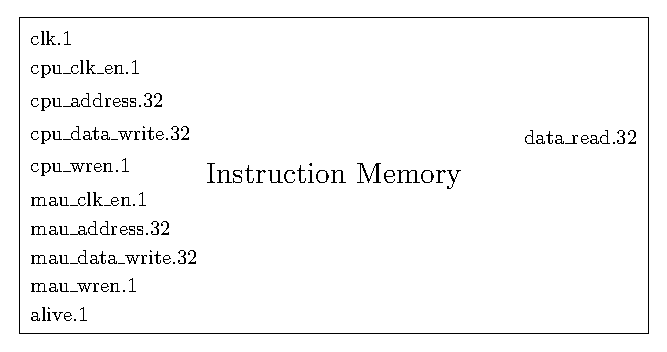
\includegraphics[scale=0.8]{Chapter3-CPU/res/instruction_memory}
    \caption{Instruction memory}
    \label{fig:components/im}
\end{figure}

In fact, a bit named alive allows the memory to choose between two buses, one that is used for 
accesses from outside the CPU (from the Memory Access Unit, this is discussed in another 
section) and one for access from the CPU. There is therefore a multiplexer on each input which
chooses one of the two buses according to the value of alive. These signals are then redirected to 
the ram\_32768 to access the memory.

\begin{figure}[H]
    \centering
    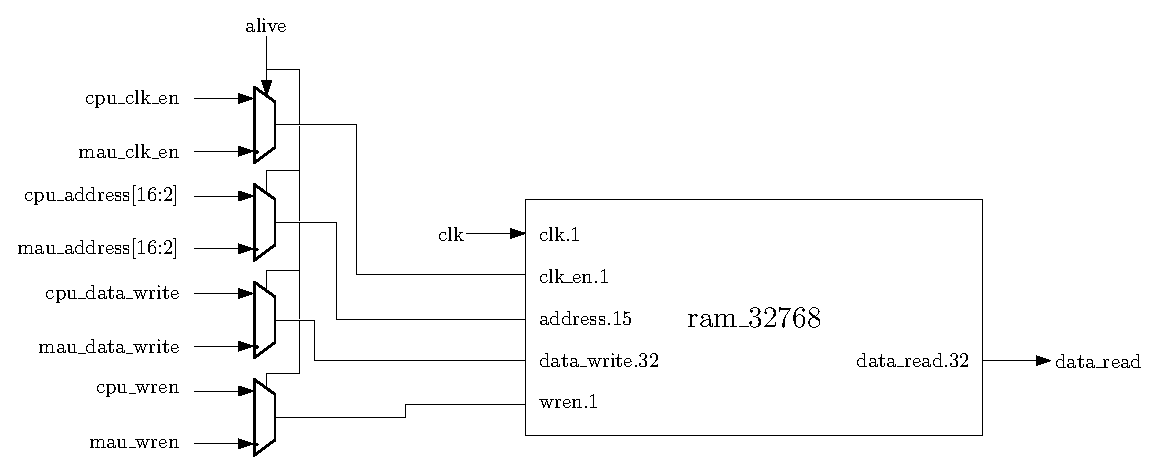
\includegraphics[width=\linewidth]{Chapter3-CPU/res/instruction_memory_in}
    \caption{Instruction memory internal circuit}
    \label{fig:components/im_in}
\end{figure}

\subsection{Data memory}

The data memory is used to store data from the CPU, it corresponds to the main memory of the CPU.

For this memory, everything happens exactly the same as for the instruction memory. The only 
thing that changes is the size of the internal RAM. Indeed, this one is 16384 words of 32bits. This 
value has been chosen to be twice as small as the instruction memory and to fit both together in 
the FPGA (in addition to the other memories that is seen later). The interface of this module
is displayed in Figure \ref{fig:components/dm} and its internal circuits in Figure \ref{fig:components/dm_in}.

\begin{figure}[H]
    \centering
    \includegraphics[scale=0.8]{Chapter3-CPU/res/data_memory}
    \caption{Data memory}
    \label{fig:components/dm}
\end{figure}

\begin{figure}[H]
    \centering
    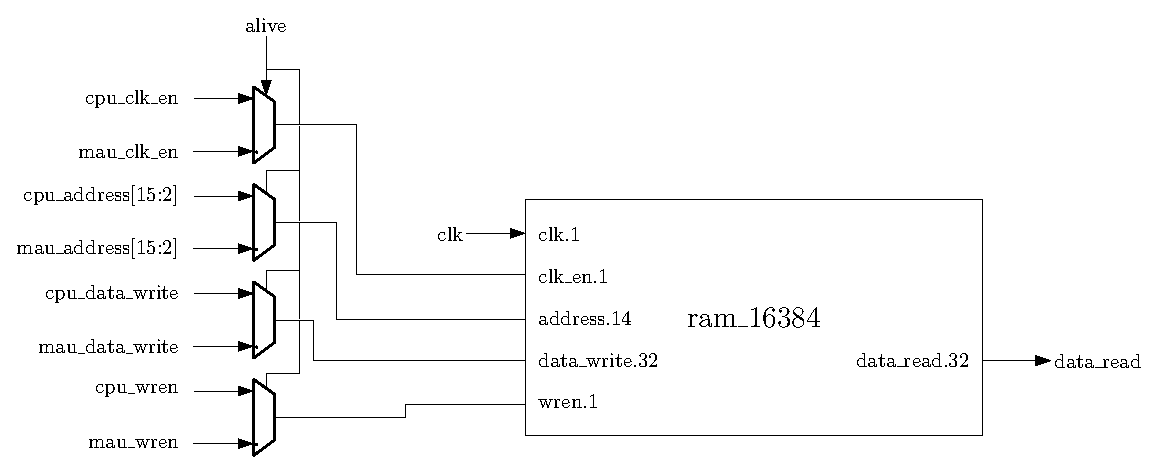
\includegraphics[width=\linewidth]{Chapter3-CPU/res/data_memory_in}
    \caption{Data memory internal circuit}
    \label{fig:components/dm_in}
\end{figure}

\subsection{Register file}

The purpose of the register file is to give access to 32 registers to the CPU. Two reads and one 
write operations must be able to be executed simultaneously by this module. A single register is not 
accessible in read mode. This is register 31. A read to this register always results in a 0
value writen on the data\_read output.

In the register file, two memories of 32 words of 32 bits are used, this memory then represents 
the 32 registers. As the register file needs two simultaneous read and write accesses, it is
mandatory to use two separate memories because Altsyncrams do not support tri-port accesses.
By having two rams with two ports, one port of each can be used to perform mirrored writes and the 
other port is used to have a read access. This gives two independent reads and a single write. In 
fact, the memories are a copy of each other in this configuration. 

However, writing and reading are never enabled at the same time in this work (the reason is explained
later in this chapter). But 
in order to provide the correct interface for future works, the register file implements all three 
ports anyway. 

Four ports are used to control the operation of the register file. First of all, the 
two clock enable signals (cpu\_clk\_en) allow reading for cpu\_clk\_en[0] and writing for cpu\_clk\_en[1].  Then, 
a cpu\_wren signal also allows to allow writing operations or not. However, in the case where the writes and 
reads of the register file are executed in two different steps, cpu\_wren and cpu\_clk\_en[1] must be in the 
high state for a write to take place. In case a user would like to use all the ports simulataneously, 
it would be required to set both cpu\_clk\_en signals to the high state. In this configuration, writing 
is then totally controlled by the cpu\_wren signal. Finally, the alive signal allows, as for the instruction and 
data memories, to make the register file listen to the CPU or MAU buses. The different ports of the register file 
are shown in Figure \ref{fig:components/rf}.

For access from the MAU, the register file exposes only one port which is used either for 
reading or writing (depending on the state of mau\_wren). That is why the mau bus only hava one 
address signal, a read signal and a write signal. When writing, the value is stored on 
both memories, while reading only operates on one memory.

\begin{figure}[H]
    \centering
    \includegraphics[scale=0.6]{Chapter3-CPU/res/reg_file}
    \caption{Register file}
    \label{fig:components/rf}
\end{figure}

As shown in Figure \ref{fig:components/rf_in}, although two memories are now present, the internal 
circuit remains very similar to that of the memories previously seen. The notable differences are at 
the level of the cpu\_clk\_en and of the cpu\_wren where the two clock enable signals 
must now be managed. At the output, a multiplexer is positioned on each of the two data-read signals in 
order to make a selection between the value in memory and 0. The value 0 is put on the output when 
the input address points to register 31.

\begin{figure}[H]
    \centering
    
\includegraphics[width=\linewidth]{Chapter3-CPU/res/reg_file_in}
    \caption{Register file internal circuit}
    \label{fig:components/rf_in}
\end{figure}

\subsection{Control logic}

The control logic is the core element of the cpu. Its purpose is to convert the opcode of an 
instruction into a set of control signals that adequately configure the different modules of 
the system so that the instruction executes properly. The control logic used in this work is simply a 
ROM (thus an Altsyncram configured in read-only mode) whose address is the opcode. The read value 
contains all control bits. As seen in the following section, the opcodes of the Beta 
machine are represented on 6 bits. The addressing of the control logic is therefore done on 6 bits. 
The words contained in the memory are represented on 12 bits.

The ROMs can be written at the compilation of the project on Quartus. This is done by associating a
hexadecimal file (.hex) to the ROM. The configuration of this file and the meaning of the different 
bits of the words in this memory are explained later in the report. 

This module being a wrapper of the Altsyncram configured in ROM, only the interface of this 
module is given, in Figure \ref{fig:components/cl}.

\begin{figure}[H]
    \centering
    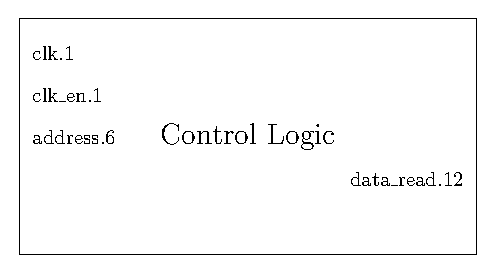
\includegraphics[scale=1]{Chapter3-CPU/res/control_logic}
    \caption{Control logic}
    \label{fig:components/cl}
\end{figure}

\subsection{Clock controller}

As mentioned earlier, the different modules making up the machine are executed in sequence and not 
in parallel. This allows to avoid pipelining in the machine and to simplify its realization. The 
execution of an instruction thus takes seven clock cycles. Pipelining could be a very interesting 
and useful subject for future works. 

For this sequence to be realized, the modules must be executed in the right order. It is therefore 
important to have a module that generates the sequence. This module is the clock\_controller. It
generates a signal named clk\_sequence which contains the seven clk\_enable signals which are 
necessary for the realization of the machine. The interface of the clock\_controller is given in
Figure \ref{fig:components/cc}. 

\begin{figure}[H]
    \centering
    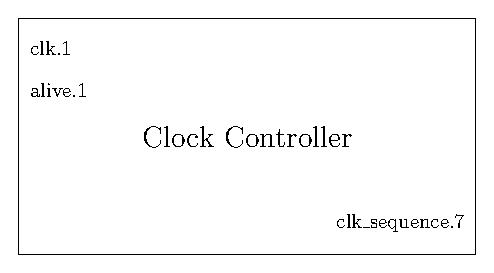
\includegraphics[scale=0.8]{Chapter3-CPU/res/clock_controller}
    \caption{Clock controller}
    \label{fig:components/cc}
\end{figure}

At the level of the realization, this module is very simple, it initializes a register to 
$0b0000001$ when the alive signal is low, then when alive is high, it carries out a circular logical 
left shift at each clock cycle. Thus, only one bit of the clk\_sequence signal is high at a time, 
and thus only one module is activated. The internal circuits of this module are shown in Figure 
\ref{fig:components/cc_in}. It is then sufficient to associate the generated signal with the clk\_en 
signals of the different modules in the right order to obtain the expected execution sequence.

\begin{figure}[H]
    \centering
    \includegraphics[scale=1.0]{Chapter3-CPU/res/clock_controller_in}
    \caption{Clock controller internal circuit}
    \label{fig:components/cc_in}
\end{figure}


\section{Instruction Set Architecture}
\subsection{Instructions formats}

Two instruction formats are used in the instruction set, the first one is used for all instructions 
requiring two operands ($R_a$ and $R_b$ in Figure \ref{fig:instructions/format}) which is for example 
the case for simple arithmetic instructions. The second format is used for all instructions 
requiring a single operand and a constant. This is the case for example for conditional jump 
operations. As can be seen in Figure \ref{fig:instructions/format}, the $R_x$ contain register 
addresses. As they are on 5 bits and no bank change operation exists, 32 registers are addressable. 
$R_c$ stores the result of the instruction when a result exists. It should be noted that the 
constants are on 16 bits and signed. In Figure \ref{fig:memories/altsyncram} the most general interface 
with two true ports is shown. 

\begin{figure}[H]
    \centering
    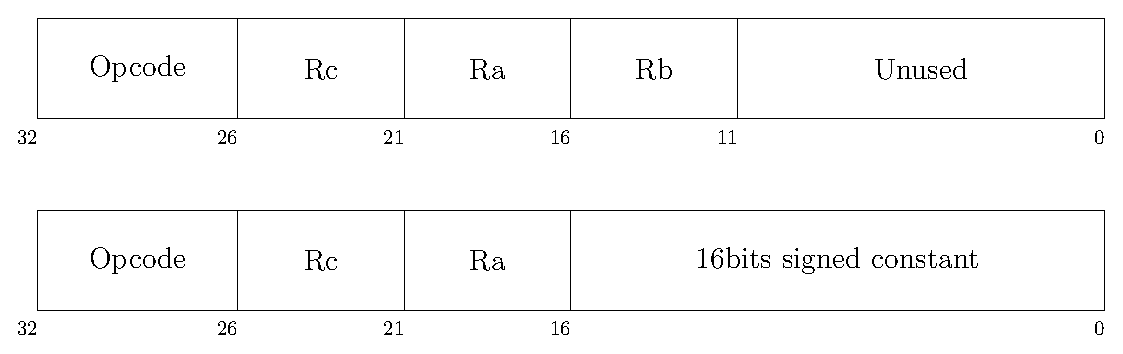
\includegraphics[scale=0.6]{Chapter3-CPU/res/instruction}
    \caption{Instructions format}
    \label{fig:instructions/format}
\end{figure}

\subsection{Instruction set}

\subsubsection*{Arithmetic and logic instructions}

The different arithmetic and logic instructions are managed by the Arithmetic Logic Unit (ALU). The 
different instructions listed in Table \ref{tab:instruction/alu} are supported.

\begin{table}[H]
    \centering
    \begin{tabular}{|l|l|l|l|l|}
    \hline
    \rowcolor[HTML]{DAE8FC} 
    \multicolumn{1}{|c|}{\cellcolor[HTML]{DAE8FC}\textbf{Name}} & \multicolumn{1}{c|}{\cellcolor[HTML]{DAE8FC}\textbf{Operation}} & \multicolumn{1}{c|}{\cellcolor[HTML]{DAE8FC}\textbf{Opcode}} & \multicolumn{1}{c|}{\cellcolor[HTML]{DAE8FC}\textbf{Const Operation}} & \multicolumn{1}{c|}{\cellcolor[HTML]{DAE8FC}\textbf{Const Opcode}} \\ \hline
    Addition                                                    & ADD                                                             & 0x20                                                         & ADDC                                                                  & 0x30                                                               \\ \hline
    Substraction                                                & SUB                                                             & 0x21                                                         & SUBC                                                                  & 0x31                                                               \\ \hline
    Multiplication                                              & MUL                                                             & 0x22                                                         & MULC                                                                  & 0x32                                                               \\ \hline
    Bitwise and                                                 & AND                                                             & 0x28                                                         & ANDC                                                                  & 0x38                                                               \\ \hline
    Bitwise or                                                  & OR                                                              & 0x29                                                         & ORC                                                                   & 0x39                                                               \\ \hline
    Bitwise xor                                                 & XOR                                                             & 0x2A                                                         & XORC                                                                  & 0x3A                                                               \\ \hline
    Compare equal                                               & CMPEQ                                                           & 0x24                                                         & CMPEQC                                                                & 0x3A                                                               \\ \hline
    Compare less                                                & CMPLT                                                           & 0x25                                                         & CMPLTC                                                                & 0x35                                                               \\ \hline
    Compare less or equal                                       & CMPLE                                                           & 0x26                                                         & CMPLEC                                                                & 0x36                                                               \\ \hline
    Logical left shift                                          & SHL                                                             & 0x2C                                                         & SHLC                                                                  & 0x3C                                                               \\ \hline
    Logical right shift                                         & SHR                                                             & 0x2D                                                         & SHRC                                                                  & 0x3D                                                               \\ \hline
    Arithmetic rifht shift                                      & SRA                                                             & 0x2E                                                         & SRAC                                                                  & 0x3E                                                               \\ \hline
    \end{tabular}
    \caption{Arithmetic and logic instructions}
    \label{tab:instruction/alu}
\end{table}

All these instructions simply perform the operation associated with them on the operands $R_a$ and 
$R_b$ in the normal case and on the operands $R_a$ and the constant in the case of instructions 
with constants. $R_a$ is always used as the first operand. For example, the instruction given 
in Figure \ref{fig:instructions/subc} results in $[R_{10}] = [R_{14}] - 17$. The notation 
$[R_x]$ means the content of register $R_x$.

\begin{figure}[H]
    \centering
    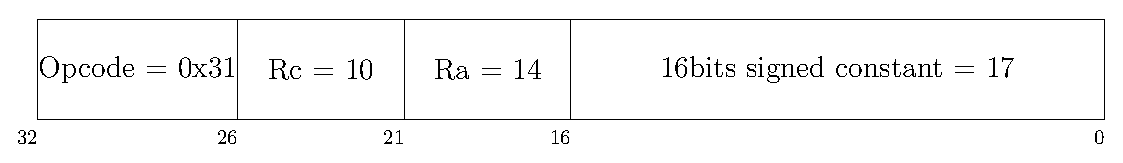
\includegraphics[scale=0.6]{Chapter3-CPU/res/instruction_subc}
    \caption{SUBC instruction example}
    \label{fig:instructions/subc}
\end{figure}

Concerning the comparison operations, they are simply put a $0$ in $R_c$ when the comparison is 
false, a $1$ otherwise.

\subsubsection*{Memory instructions}

Here, only two instructions are present. One is to load a value from the data memory and the other 
is to store a value in it. The notation $<x>$ means at address $x$ in memory. Note that here $R_c$
doesn't necessarily contains a result at the end of an operation and is used as an operand for ST.
Also, addresses must be byte aligned here and offsets contained in Constant must also be byte
aligned. Both instructions are detailed in Table \ref{tab:instruction/dm}.

\begin{table}[H]
    \centering
    \begin{tabular}{|l|l|l|l|}
    \hline
    \rowcolor[HTML]{DAE8FC} 
    \multicolumn{1}{|c|}{\cellcolor[HTML]{DAE8FC}\textbf{Name}} & \multicolumn{1}{c|}{\cellcolor[HTML]{DAE8FC}\textbf{Operation}} & \multicolumn{1}{c|}{\cellcolor[HTML]{DAE8FC}\textbf{Opcode}} & \multicolumn{1}{c|}{\cellcolor[HTML]{DAE8FC}\textbf{Action}} \\ \hline
    Load                                                        & LD                                                              & 0x18                                                         & {[}Rc{]} = $<${[}Ra{]} + Constant$>$      \\ \hline
    Store                                                       & ST                                                              & 0x19                                                         & $<${[}Ra{]} + Constant$>$ = {[}Rc{]}        \\ \hline
    \end{tabular}
    \caption{Memory instructions}
    \label{tab:instruction/dm}
\end{table}

\subsubsection*{Program counter instructions}

The purpose of these instructions is to modify the value of the program counter conditionally or 
not. The different instructions are listed in Table \ref{tab:instruction/pc}. The values of 
column Next PC is writen to PC and the address of the next instruction before the jump is
stored in Rc. Note that [Ra] should be byte aligned for JMP but the constant should be 32bits 
aligned for BEQ and BNE (as they already multiply the constant by 4).

\begin{table}[H]
    \centering
    \begin{tabular}{|l|l|l|l|l|}
    \hline
    \rowcolor[HTML]{DAE8FC} 
    \multicolumn{1}{|c|}{\cellcolor[HTML]{DAE8FC}\textbf{Name}} & \multicolumn{1}{c|}{\cellcolor[HTML]{DAE8FC}\textbf{Operation}} & \multicolumn{1}{c|}{\cellcolor[HTML]{DAE8FC}\textbf{Opcode}} & \multicolumn{1}{c|}{\cellcolor[HTML]{DAE8FC}\textbf{Condition}} & \multicolumn{1}{c|}{\cellcolor[HTML]{DAE8FC}\textbf{Next PC}} \\ \hline
    Jump                                                        & JMP                                                             & 0x1B                                                         & None                                                                 & {[}Ra{]} \& 0xFFFFFFC                                         \\ \hline
    Branch Equal                                                & BEQ                                                             & 0x1D                                                         & {[}Ra{]} == 0                                                        & PC + 4 $\times$ (Constant + 1)             \\ \hline
    Branch Not Equal                                            & BNE                                                             & 0x1E                                                         & {[}Ra{]} != 0                                                        & PC + 4 $\times$ (Constant + 1)                \\ \hline
    \end{tabular}
    \caption{Program counter instructions}
    \label{tab:instruction/pc}
\end{table}

\subsubsection*{Control instructions}

Only one control instruction exists. This instruction bascally stops the machine and has no operand
or result. The instruction is detailed in Table \ref{tab:instruction/ctrl}

\begin{table}[H]
    \centering
    \begin{tabular}{|l|l|l|}
    \hline
    \rowcolor[HTML]{DAE8FC} 
    \multicolumn{1}{|c|}{\cellcolor[HTML]{DAE8FC}\textbf{Name}} & \multicolumn{1}{c|}{\cellcolor[HTML]{DAE8FC}\textbf{Operation}} & \multicolumn{1}{c|}{\cellcolor[HTML]{DAE8FC}\textbf{Opcode}} \\ \hline
    Exit                                                        & EXIT                                                            & 0x3F                                                         \\ \hline
    \end{tabular}
    \caption{Exit instruction}
    \label{tab:instruction/ctrl}
\end{table}

\section{Beta machine}

The final circuit of the beta machine is shown in Figure \ref{fig:beta/all}. The details of this 
circuit and how the modules have been interconnected are explained in this section. 

\begin{figure}[H]
    \centering
    
\includegraphics[width=\linewidth]{Chapter3-CPU/res/beta_machine_in}
    \caption{Beta machine internal circuit}
    \label{fig:beta/all}
\end{figure}

\subsection{Modules sequence}

The first thing to establish is the execution sequence.  The first step is to fetch an instruction 
from the memory instruction, so it is executed first. Then, the opcode of this instruction must be 
decoded by the control logic. The control logic has the second position. The register file can now 
be executed in read mode, in order to obtain the values of the registers useful in the current 
instruction. This step could not have been carried out at the same time as the previous one because 
a multiplexer controlled by a signal from the control logic is present at the cpu\_read\_address\_2 
input of the Register File. This allows it to choose between Rb and Rc, Ra always being the address 
of the first port. 

The values of the registers are now present at the output of the Register file, the ALU is then 
executed. In case the result of the ALU should be stored in Data memory, it is then executed. Also, when 
executing the Data memory, it could provide data that must be stored in a register. That is why the 
next step is the execution of the Register file in write mod. Finally, the Program counter is enabled 
so that the PC is updated. The execution sequence is displayed in Figure \ref{fig:beta/sequence}.

\begin{figure}[H]
    \centering
    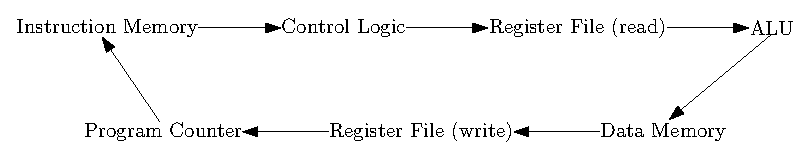
\includegraphics[scale=0.8]{Chapter3-CPU/res/sequence}
    \caption{Execution sequence}
    \label{fig:beta/sequence}
\end{figure}

\subsection{Instructions and control logic}

In this section, the content of the control logic is defined. At the same time, the connections 
between the different modules forming the Beta machine are also explained. The complete circuit of 
the Beta machine is shown in Figure \ref{fig:beta/all}. The reader can refer to it to follow the 
developments of this section.

First of all, the output pc\_next of the program counter is connected to its input pc\_in to form a 
counter by 4. The output pc\_out of the program counter can be connected to the CPU address of the 
memory instruction in order to read the current instruction. The first six bits of this instruction 
are connected to the address of the control logic so that the opcode is decoded. Of course, the clk 
and clk\_enable signals of all modules are also set to follow the sequence described in the previous 
section.

\subsubsection*{Arithmetic and logic instructions}

In order for an ALU instruction to perform correctly, two things are required. Firstly, that the 
necessary registers are read from the register file and secondly that the ALU executes the operation. 
To do this, the instruction coming from the instruction memory is split. The bits corresponding to 
Ra go to the address of the first port and the bits corresponding to Rb to the second port. As the 
results are stored in the register Rc, the bits corresponding to Rc in the instruction are 
used as the write address for the register file. The two operand registers can then be loaded. 

For the ALU, it needs on its first input the value read in the register Ra, this is why the reading 
of the first port directly goes to the first input of the ALU. As for the second operand of the ALU, 
it can either be the value of Rb or a constant. This is why a multiplexer is placed on the input 
corresponding to the second operand. Finally, the result of the ALU is redirected to the register 
file so that it can store this value in Rc.

At the control logic level, three signals are necessary. The first is used to control the operation 
of the ALU, it is alufn. The second is bsel and allows to choose if the second operand of the ALU 
is the constant or the value read in register Rb. And lastly, the signal werf allows to 
authorize the write operation in the register file. The current content of the control logic is 
shown in Table \ref{tab:cl/alu}.

\begin{table}[H]
    \centering
    \begin{tabular}{|l|c|c|c|}
    \hline
    \rowcolor[HTML]{DAE8FC} 
    \multicolumn{1}{|c|}{\cellcolor[HTML]{DAE8FC}\textbf{Instruction}} & \textbf{alufn} & \textbf{werf} & \textbf{bsel} \\ \hline
    ALU instruction                                                    & opcode         & 1             & 1             \\ \hline
    ALU constant instruction                                           & opcode         & 1             & 0             \\ \hline
    \end{tabular}
    \caption{Control logic - ALU instructions}
    \label{tab:cl/alu}
\end{table}

\subsubsection*{Memory instructions}

As shown in Table \ref{tab:instruction/dm}, the load operation (LD) executes [Rc] = $<$[Ra] + constant$>$.
To make this operation possible, a sum with constant must be performed and its result used as an 
address for the data memory. This is why the output of the ALU is set as an address for the data 
memory. Then the value read from the data memory must be used as a write value to the register file. 
As a signal has already been connected to this register file entry, a multiplexer must be added 
which chooses between the ALU output and the value read from the data memory.

Concerning the control logic, a signal named wdsel is added to drive the newly added multiplexer.

For the storage operation in data memory (ST), $<$[Ra] + constant$>$ = [Rc] must be executed.
Everything remains the same as for the load at the ALU and the first port of the register file. 
However, the value in Rc must be read in the register file and nothing allows it until now. As Ra is 
already using the first port, Rc is put on the second port for reading. A multiplexer must be added 
to it as Rb was already associated with this port. The output of the second port of the register 
file must be connected to the cpu\_data\_write input of the data memory so that [Rc] is written 
there. 

Two new signals are added to the control logic. The first, wr, allows the data memory to be written 
and the second, ra2sel, drives the multiplier which has just been added. The current content of the 
logical control is displayed in Table \ref{tab:cl/dm}.

\begin{table}[H]
    \centering
    \begin{tabular}{|l|c|c|c|c|c|c|}
    \hline
    \rowcolor[HTML]{DAE8FC} 
    \multicolumn{1}{|c|}{\cellcolor[HTML]{DAE8FC}\textbf{Instruction}} & \textbf{alufn} & \textbf{werf} & \textbf{bsel} & \multicolumn{1}{l|}{\cellcolor[HTML]{DAE8FC}\textbf{wdsel}} & \multicolumn{1}{l|}{\cellcolor[HTML]{DAE8FC}\textbf{wr}} & \multicolumn{1}{l|}{\cellcolor[HTML]{DAE8FC}\textbf{ra2sel}} \\ \hline
    ALU instruction                                                    & opcode         & 1             & 1             & 01                                                          & 0                                                        & 0                                                            \\ \hline
    ALU constant instruction                                           & opcode         & 1             & 0             & 01                                                          & 0                                                        & x                                                            \\ \hline
    Load instruction                                                   & add            & 1             & 0             & 10                                                          & 0                                                        & x                                                            \\ \hline
    Store instruction                                                  & add            & 0             & 0             & xx                                                          & 1                                                        & 1                                                            \\ \hline
    \end{tabular}
    \caption{Control logic - ALU and memory instructions}
    \label{tab:cl/dm}
\end{table}

\subsubsection*{Program counter instructions}

For the JMP instruction, it is first necessary to save the value of PC + 4 in Rc. This means that 
the output pc\_next of the program counter must be able to be used as a write value for the register 
file. pc\_nect is therefore added to the multiplexer driven by wdsel. Then, the value of PC must be 
set to the value given in Ra. The reading of the first port of the register file is therefore 
connected to the data port of the register file. The register file must also be set to JMP mode.

Only one signal must be added to the control logic, this is the pcsel which will allow the program 
counter mode to be set.

For the branch instructions, everything happens as for JMP except that the value of pc is different 
in the control logic and that the constant contained in the instruction is connected to the offset 
input of the program counter.. The final content of the control logic is given in Table \ref{tab:cl/all}.

\begin{table}[H]
    \centering
    \begin{tabular}{|l|c|c|c|c|c|c|c|}
    \hline
    \rowcolor[HTML]{DAE8FC} 
    \multicolumn{1}{|c|}{\cellcolor[HTML]{DAE8FC}\textbf{Instruction}} & \textbf{alufn} & \textbf{werf} & \textbf{bsel} & \textbf{wdsel} & \textbf{wr} & \textbf{ra2sel} & \textbf{pc} \\ \hline
    ALU instruction                                                    & opcode         & 1             & 1             & 01             & 0           & 0               & 00          \\ \hline
    ALU constant instruction                                           & opcode         & 1             & 0             & 01             & 0           & x               & 00          \\ \hline
    Load instruction                                                   & add            & 1             & 0             & 10             & 0           & x               & 00          \\ \hline
    Store instruction                                                  & add            & 0             & 0             & xx             & 1           & 1               & 00          \\ \hline
    JMP instruction                                                    & xxxx           & 1             & x             & 00             & 0           & x               & 10          \\ \hline
    BEQ instruction                                                    & xxxx           & 1             & x             & 00             & 0           & x               & 01          \\ \hline
    BNE instruction                                                    & xxxx           & 1             & x             & 00             & 0           & x               & 11          \\ \hline
    \end{tabular}
    \caption{Control logic - ALU, memory and program counter instructions}
    \label{tab:cl/all}
\end{table}

In the control logic, all values corresponding to don't care (x), are set to 0. 

\subsubsection*{Control instructions}

The last instruction to be handled is EXIT which is intended to generate a halt signal. As the EXIT 
instruction corresponds to opcode 0x3F, it is sufficient to put all the bits of the opcode at the 
input of an AND logic gate in order to have at the output the halt signal which will be high when 
EXIT is called.

\subsection{Other signals and ports}

The Beta machine is only part of the system designed during this work. In fact, it consists of the 
CPU of this system. It therefore has other ports which allow its connection with other super-modules. 

First there are the four ports exported\_address, exported\_data, exported\_wren and io\_data,
the first three allow to add listeners to the ST instruction. io\_data allows, with the 
three signals mentioned above, to add the IO unit (IOU) as a listener to the LD instruction. In the 
context of this work, the first two bits of the address are used to designate the listener which 
is concerned by the ST and LD operations. For the LD part, it is therefore necessary to add a 
multiplexer before putting the result of a data memory load on the multiplexer controlled by wdsel. 
The purpose of this multiplexer is to select where the load comes from. io\_data therefore 
constitutes an input of this multiplexer. The addressing table for the different units is described 
in Table \ref{tab:beta/address}. 

\begin{table}[H]
    \centering
    \begin{tabular}{|l|c|}
    \hline
    \rowcolor[HTML]{DAE8FC} 
    \multicolumn{1}{|c|}{\cellcolor[HTML]{DAE8FC}\textbf{Super unit}} & \textbf{Address} \\ \hline
    CPU                                                               & 00               \\ \hline
    IOU                                                               & 01               \\ \hline
    GPU                                                               & 10               \\ \hline
    \end{tabular}
    \caption{Super unit addresses}
    \label{tab:beta/address}
\end{table}

Then, there are the halt and alive signals. These two signals allow communication with the control 
unit (CTRLU), their use is discussed later.

Finally, there are all the signals starting with mau. These are connected to the Memory Access Unit 
(MAU). Again, this unit is seen later in the report. 

In the end, this gives the CPU a more complex interface than usual. This interface is that of 
Figure \ref{fig:beta/interface}. In order to simplify the CPU interface, not all signals are put in 
the CPU and a bus representation is used. However, all signals are available in the internal circuit.

\begin{figure}[H]
    \centering
    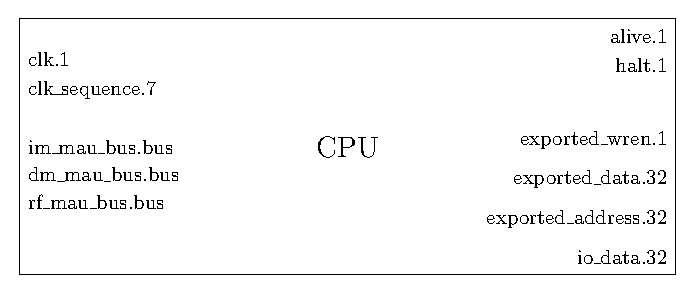
\includegraphics[scale=0.8]{Chapter3-CPU/res/beta_machine}
    \caption{Beta machine, the CPU}
    \label{fig:beta/interface}
\end{figure}